\documentclass[11pt]{charter}

% El títulos de la memoria, se usa en la carátula y se puede usar el cualquier lugar del documento con el comando \ttitle
\titulo{Diseño de un indicador de peso de gama media} 

% Nombre del posgrado, se usa en la carátula y se puede usar el cualquier lugar del documento con el comando \degreename
\posgrado{Carrera de Especialización en Sistemas Embebidos} 
%\posgrado{Carrera de Especialización en Internet de las Cosas} 
%\posgrado{Carrera de Especialización en Intelegencia Artificial}
%\posgrado{Maestría en Sistemas Embebidos} 
%\posgrado{Maestría en Internet de las cosas}

% Tu nombre, se puede usar el cualquier lugar del documento con el comando \authorname
\autor{Sanchez Gonzalo Daniel} 

% El nombre del director y co-director, se puede usar el cualquier lugar del documento con el comando \supname y \cosupname y \pertesupname y \pertecosupname
\director{Ezequiel Marengo}
\pertenenciaDirector{Sipel S.R.L.} 
% FIXME:NO IMPLEMENTADO EL CODIRECTOR ni su pertenencia
\codirector{} % si queda vacio no se deberíá incluir 
\pertenenciaCoDirector{}

% Nombre del cliente, quien va a aprobar los resultados del proyecto, se puede usar con el comando \clientename y \empclientename
\cliente{Ivan Barenboim}
\empresaCliente{Sipel S.R.L.}

% Nombre y pertenencia de los jurados, se pueden usar el cualquier lugar del documento con el comando \jurunoname, \jurdosname y \jurtresname y \perteunoname, \pertedosname y \pertetresname.
\juradoUno{Nombre y Apellido (1)}
\pertenenciaJurUno{pertenencia (1)} 
\juradoDos{Nombre y Apellido (2)}
\pertenenciaJurDos{pertenencia (2)}
\juradoTres{Nombre y Apellido (3)}
\pertenenciaJurTres{pertenencia (3)}
 
\fechaINICIO{23 de octubre de 2020}		%Fecha de inicio de la cursada de GdP \fechaInicioName
\fechaFINALPlanificacion{13 de octubre de 2020} 	%Fecha de final de cursada de GdP
\fechaFINALTrabajo{11 de diciembre de 2021}		%Fecha de defensa pública del trabajo final


\begin{document}

\maketitle
\thispagestyle{empty}
\pagebreak


\thispagestyle{empty}
{\setlength{\parskip}{0pt}
\tableofcontents{}
}
\pagebreak


\section{Registros de cambios}
\label{sec:registro}


\begin{table}[ht]
\label{tab:registro}
\centering
\begin{tabularx}{\linewidth}{@{}|c|X|c|@{}}
\hline
\rowcolor[HTML]{C0C0C0} 
Revisión & \multicolumn{1}{c|}{\cellcolor[HTML]{C0C0C0}Detalles de los cambios realizados} & Fecha      \\ \hline
1.0      & Creación del documento                                          & 23/10/2020 \\ \hline
1.1      & Se agregan historias de usuario y se corrigen observaciones a la primer entrega                                 & 13/11/2020 \\ \hline
1.2      & Se agregan secciones 7 a 11 & 22/11/2020\\ \hline
1.3      & Se agregan secciones 12 a 17  \newline
 Se corrigen observaciones realizadas a las versiones 1.1 y 1.2 & xx/12/2020 \\ \hline
1.4      & Se agregan secciones 12 a 17 & 03/12/2020\\ \hline 
%		   Con texto partido \newline
%		   En varias líneas \newline
%		   A propósito                                                     & dd/mm/aaaa \\ \hline
\end{tabularx}
\end{table}

\pagebreak



\section{Acta de constitución del proyecto}
\label{sec:acta}

\begin{flushright}
Buenos Aires, \fechaInicioName
\end{flushright}

\vspace{2cm}

Por medio de la presente se acuerda con el Ing. \authorname\hspace{1px} que su Trabajo Final de la \degreename\hspace{1px} se titulará ``\ttitle'', consistirá esencialmente en la selección de la tecnología adecuada, el diseño de los circuitos esquemáticos y la generación del código fuente necesario para el desarrollo de una nueva familia de indicadores y controladores de peso que reemplace a familia de indicadores de gama media que la empresa Sipel S.R.L. fabrica y comercializa actualmente. También se generará la documentación pertinente para realizar una transferencia tecnológica que le permita a la empresa el posterior mantenimiento o modificación del producto final. El código fuente generado será testeado sobre un prototipo cuya construcción estará a cargo de la empresa o en su defecto sobre una plataforma de desarrollo (development kit) acorde a la tecnología seleccionada para el diseño. El proyecto tendrá un presupuesto preliminar estimado de 670 hs de trabajo y \textcolor{red}{\$826.000}, con fecha de inicio \fechaInicioName\hspace{1px} y fecha de presentación pública \fechaFinalName.

Se adjunta a esta acta la planificación inicial.

\vfill

% Esta parte se construye sola con la información que hayan cargado en el preámbulo del documento y no debe modificarla
\begin{table}[ht]
\centering
\begin{tabular}{ccc}
\begin{tabular}[c]{@{}c@{}}Ariel Lutenberg \\ Director posgrado FIUBA\end{tabular} & \hspace{2cm} & \begin{tabular}[c]{@{}c@{}}\clientename \\ \empclientename \end{tabular} \vspace{2.5cm} \\ 
\multicolumn{3}{c}{\begin{tabular}[c]{@{}c@{}} \supname \\ Director del Trabajo Final\end{tabular}} \vspace{2.5cm} \\
%\begin{tabular}[c]{@{}c@{}}\jurunoname \\ Jurado del Trabajo Final\end{tabular}     &  & \begin{tabular}[c]{@{}c@{}}\jurdosname\\ Jurado del Trabajo Final\end{tabular}  \vspace{2.5cm}  \\
%\multicolumn{3}{c}{\begin{tabular}[c]{@{}c@{}} \jurtresname\\ Jurado del Trabajo Final\end{tabular}} \vspace{.5cm}                                                                     
\end{tabular}
\end{table}




\section{Descripción técnica-conceptual del proyecto a realizar}
\label{sec:descripcion}

%\begin{consigna}{red}
%El objetivo es que el lector en una o dos páginas entienda de qué se trata el proyecto y cuáles son sus desafíos, su motivación y su importancia.
%Se debe destacar claramente cuál es el valor que agrega el proyecto a realizar. ``El presente proyecto se destaca especialmente por incorporar tal cosa... Esto lo diferencia de otros sistemas similares en que ...''
%
%Puede ser útil incluir en esta sección la respuesta a alguna de estas preguntas:
%
%\begin{itemize}
%\item ¿Cómo se vincula este proyecto con la misión de la organización?
%\item ¿Cómo se inserta este proyecto en el modelo de negocio de la organización?
%\item ¿Ayuda a la explicación si se incluye un lienzo Canvas del Modelo de Negocio?
%\item ¿En qué estado del ciclo de vida está el producto que se desea reemplazar o mejorar?
%\item ¿Cuales son las necesidades que debe satisfacer?
%\item ¿Por dónde pasa la innovación?
%\end{itemize}
%
%La descripción técnica-conceptual \textbf{debe incluir al menos un diagrama en bloques del sistema }y una frase como la siguiente: ``En la Figura \ref{fig:diagBloques} se presenta el diagrama en bloques del sistema. Se observa que...''. Luego recién más abajo de haber puesto esta frase se pone la figura. La regla es que las figuras nunca pueden ir antes de ser mencionadas en el texto, porque sino el lector no entiende por qué de pronto aparece una figura.
%
%\vspace{25px}
%
%\begin{figure}[htpb]
%\centering 
%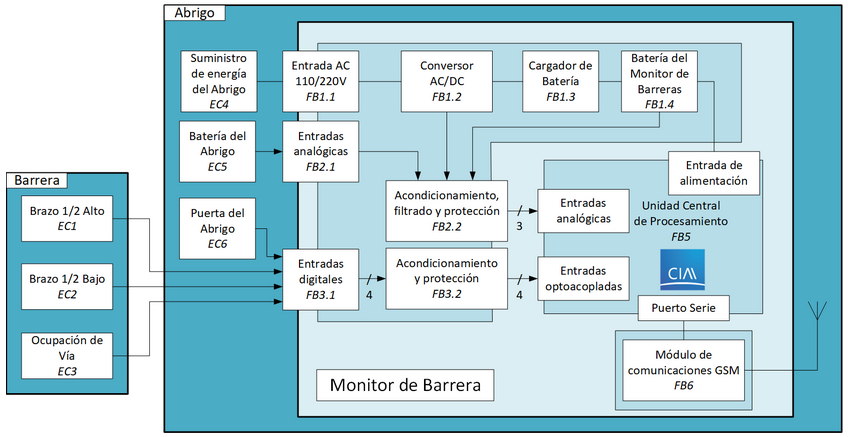
\includegraphics[width=.7\textwidth]{./Figuras/diagBloques.png}
%\caption{Diagrama en bloques del sistema}
%\label{fig:diagBloques}
%\end{figure}
%
%\vspace{25px}
%
%El tamaño de la tipografía en la figura debe ser adecuado para que NO pase lo que ocurre acá, donde el lector debe esforzarse para poder leer el texto. Los colores usados en el diagrama deben ser adecuados, tal que ayuden a comprender mejor el diagrama.
%\end{consigna}

En los recientes años la empresa Sipel S.R.L. comenzó a reemplazar su gama de indicadores de peso basados en procesadores de 8 bits por nuevos modelos basados en procesadores de 32 bits con el objetivo de ofrecer mayores prestaciones y a menor costo. Durante este proceso se diseñaron y lanzaron al mercado dos nuevos modelos de indicadores, el indicador de tope de gama “Onix” (\url{https://www.sipel.com.ar/es/producto/onix}) y el indicador de peso NEO (\url{https://www.sipel.com.ar/es/producto/neo}) como indicador de entrada de gama mientras que los indicadores de peso de gama media ORION y ATLAS  aún están basados en procesadores de 8 bits y deben ser rediseñados.\\

Habiendo lanzado al mercado los equipos NEO y ONIX y se realizó un estudio de mercado con el cual la empresa ha concluido que el mercado de indicadores de baja gama o de entrada de gama (NEO) es un mercado poco competitivo y saturado por equipos de bajo costo principalmente provenientes de China. También se concluyó  que estos equipos son poco requeridos en el mercado de pesaje industrial, el cual es el principal nicho de mercado de interés de la empresa. En este contexto la empresa plantea la necesidad de diseñar un nuevo equipo que fusione el costo competitivo de la línea de baja gama con las prestaciones de los equipos de media gama y así terminar de modernizar toda la familia de indicadores de peso de la empresa. De dicho estudio  también se desprendió la necesidad de dotar a los nuevos dispositivos con funcionalidades de conexión Wi-Fi y funcionalidades IoT de crecientes demanda en el mercado.\\

Los indicadores de peso son instrumentos de medición que conectados a un receptor de carga conforman una balanza o instrumento de pesaje. Los receptores de carga normalmente se basan en celdas de carga las cuales son piezas metálicas con Galgas extensiométricas pegadas a ellas y que al sufrir una deformación mecánica por una fuerza aplicada varían la resistencia eléctrica de manera aproximadamente lineal a la fuerza aplicada. Todas las celdas de carga comerciales tienen aproximadamente el mismo rango de tensión de alimentación, similares impedancias de las galgas y por ende similares rangos señal de salida independientemente de su capacidad de peso (máxima fuerza aplicada admitida), lo que permite que un mismo indicador de peso debidamente diseñado pueda ser conectado diversas configuraciones de receptores de carga con diversas capacidades de peso máximo y distintas apreciaciones. De esta manera, el mismo equipo electrónico puede ser utilizado en diversas aplicaciones de pesaje industriales y/o comerciales según a qué tipo de receptor de carla sea conectado.


Genéricamente un indicador de peso digital tiene los siguiente bloques constitutivos:
\begin{itemize} 
\item[•] Una fuente regulada de tensión para alimentar las celdas de carga.
\item[•] Conversor análogo-digital para leer la señal proveniente de las celdas de carga (salida del puente).
\item[•] Microprocesador para convertir las cuentas de ADC a una magnitud expresada en unidades de peso (kilogramo comúnmente), manejo de display, teclado, comunicaciones, etc.
\item[•] Memoria no volátil para guardar los datos de calibración (cap. máx, incremento, cero y span) datos de configuración (configuraciones de puerto serie, etc) y totalizadores (peso total acumulado, cantidad de pesos registrados o número de ticket, etc).
\item[•] Display para mostrar la lectura del peso con indicadores de movimiento, de centro de cero y de tara tomada (indicadores obligatorios por ley en la República Argentina).
\item[•] Teclado que contiene al menos las teclas de toma de cero y de toma de tara y las que sean necesarias para la operatoria básica del equipo como ser su calibración (selección de capacidad máxima, selección de incrementó, toma de cero y toma span con pesas patrones) y configuraciones tales como parametrización del puerto serie.
\end{itemize}

En el caso particular del proyecto en cuestión, se pueden mencionar también los siguientes bloques adicionales:
\begin{itemize}
\item[•]Puerto de comunicación serie (RS232/RS485) para múltiples propósitos como ser comunicación con impresoras de ticket, comunicación con PLC’s (protocolo modbus RTU), envío de lectura de peso a PC (texto plano), etc.
\item[•]Modulo Wi-Fi para envío de información estadística a la nube o captura de peso en tiempo real  desde software online o aplicación de escritorio.
\item[•]Puerto de expansión I2C para agregado de placa opcional de manejo de entradas/salidas de potencia para comando de diversos procesos de automatismo (sirenas en modos de alto/bajo/ok, procesos de embolsado de grano, proceso de dosificado, etc).
\item[•]Módulo opcional para uso de batería interna (control de carga).
\end{itemize}

En la Figura \ref{fig:diagBloques} se muestra un diagrama simplificado con los bloques mencionados

\vspace{25px}

\begin{figure}[htpb]
\centering 
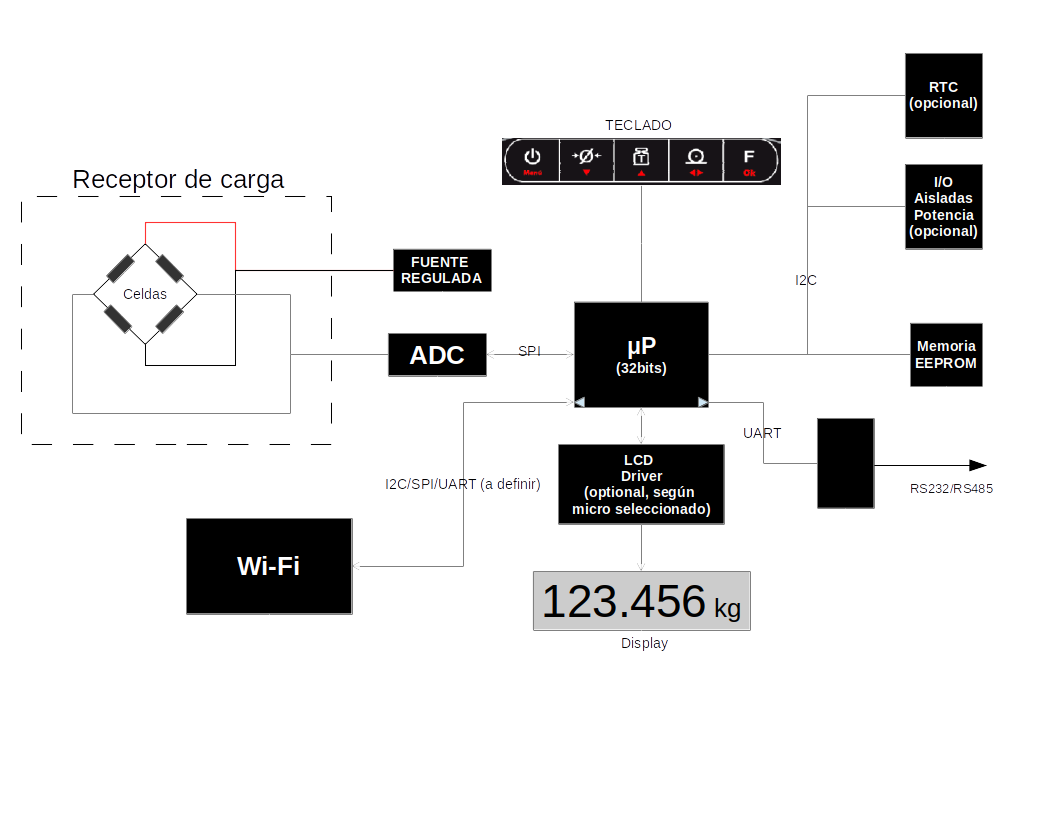
\includegraphics[width=.7\textwidth]{./Figuras/esquema.png}
\caption{Diagrama en bloques del sistema}
\label{fig:diagBloques}
\end{figure}

\vspace{25px}
\newpage
\section{Identificación y análisis de los interesados}
\label{sec:interesados}

\begin{consigna}{red} 
%Nota: (borrar esto y todas las consignas en color rojo antes de entregar este documento).
 
%Es inusual que una misma persona esté en más de un rol, incluso en proyectos chicos.
 
%Si se considera que una persona cumple dos o más roles, entonces sólo dejarla en el rol más importante. Por ejemplo:

%\begin{itemize}
%\item Si una persona es Cliente pero también colabora u orienta, dejarla solo como Cliente.
%\item Si una persona es el Responsable, no debe ser colocado también como Miembro del equipo.
%\end{itemize}

%Pero en cambio sí es usual que el Cliente y el Auspiciante sean el mismo, por ejemplo.

\begin{table}[ht]
%\caption{Identificación de los interesados}
%\label{tab:interesados}
\begin{tabularx}{\linewidth}{@{}|l|X|X|l|@{}}
\hline
\rowcolor[HTML]{C0C0C0} 
Rol           & Nombre y Apellido & Organización 	& Puesto 	\\ \hline
Auspiciante   &                   &              	&        	\\ \hline
Cliente       & \clientename      &\empclientename & CEO       	\\ \hline
Impulsor      &                   &              	&        	\\ \hline
Responsable   & \authorname       & FIUBA        	& Alumno 	\\ \hline
Colaboradores &                   &              	&        	\\ \hline
Orientador    & \supname	       & \pertesupname 	& Director	Trabajo final \\ \hline
Equipo        &                   &              	&        	\\ \hline
Opositores    &                   &              	&        	\\ \hline
Usuario final &                   &              	&        	\\ \hline
\end{tabularx}
\end{table}

%El Director suele ser uno de los Orientadores.
%
%No dejar celdas vacías; si no hay nada que poner en una celda colocar un signo ``-''.
%
%No dejar filas vacías; si no hay nada que poner en una fila entonces eliminarla.
%
%Sería deseable listar a continuación de la tabla las principales características de cada interesado.
% 
%Por ejemplo:
%\begin{itemize}
%\item Auspiciante: es riguroso y exigente con la rendición de gastos. Tener mucho cuidado con esto.
%\item Equipo: Juan Perez, suele pedir licencia porque tiene un familiar con una enfermedad. Planificar considerando esto.
%\item Orientador: María Gómez, nos va a poder ayudar mucho con la gestión de impuestos.
%\end{itemize}

\end{consigna}



\section{1. Propósito del proyecto}
\label{sec:proposito}

%\begin{consigna}{red}
%¿Por qué se hace el proyecto? ¿Qué se quiere lograr? 
%
%Se recomienda que sea solo un párrafo que empiece diciendo ``El propósito de este proyecto es...''.
%\end{consigna}

El propósito de este proyecto es asistir a la empresa Sipel S.R.L. en el desarrollo de un nuevo producto y nace de la necesidad por parte de la empresa de tercerizar parte del diseño electrónico de dicho desarrollo. Como resultado final del proyecto se pretende haber generado los esquemas electrónicos necesarios para la construcción de un prototipo, haber seleccionado las herramientas de desarrollo necesarias (compiladores, IDE, repositorios, etc.) con la documentación necesaria para su correcta instalación y uso y la generación  del código fuente que se ejecute sobre el prototipo y cumpliendo con los requerimientos funcionales del futuro producto.


\section{2. Alcance del proyecto}
\label{sec:alcance}

%\begin{consigna}{red}
%¿Qué se incluye y que no se incluye en este proyecto?
%
%Se refiere al trabajo a hacer para entregar el producto o resultado especificado. 
%
%Explicitar todo lo quede comprendido dentro del alcance del proyecto.
%
%Explicitar además todo lo que no quede incluido (``El presente proyecto no incluye...'')
%
%\end{consigna}

El presente proyecto prevé la ejecución de las siguientes tareas:
\begin{itemize}
\item[•]Seleccionar los principales componentes como ser el microcontrolador, el módulo Wi-Fi, y el display a utilizar en el diseño.
\item[•]Confeccionar los circuitos esquemáticos del producto indicando los valores y/o números de partes de los componentes. El tipo de encapsulado de cada componente y/o su marca sólo será sugerido pero la selección final quedará a cargo del responsable del diseño de circuito impreso salvo casos donde dicha selección sea crítica y se especifique puntualmente. 
\item[•]También se podrán indicar, sólo en caso de ser necesario, pautas para el diseño del PCB como ser impedancias características de      pistas, distribución sugerida de los componentes  por consideraciones de compatibilidad electromagnética o en caso de existir más de un PCB precauciones a tomar en el interconexionado de los mismos. 
\item[•]Desarrollo y testeo del código fuente del microprocesador y del módulo Wi-Fi en caso de seleccionarse un módulo programable. 
\item[•]Generar la documentación correspondiente a los ítems anteriores.
\item[•]Generar una transferencia tecnológica que le permita a la empresa asimilar y reutilizar toda nueva tecnología que se emplee en el diseño. 
\end{itemize}


Quedarán excluidas del proyecto y a cargo de Sipel S.R.L. las siguientes tareas:
\begin{itemize}
\item[•]Diseño del/los circuito(s) impreso(s) y la selección final de los encapsulados de los componentes a utilizar salvo casos  donde hayan sido expresamente indicados. Durante el diseño del PCB se podrá generar un proceso iterativo de      revisión y rediseño de los esquemáticos siempre que sea necesario.
\item[•]Diseño estético y de gabineteria del equipo.
\item[•]Realizar los dos ítems anteriores con las consideraciones necesarias para que el equipo pueda aprobar satisfactoriamente los ensayos electromagnéticos requeridos para su aprobación legal.
\item[•]Realizar los ensayos metrológicos y de compatibilidad electromagnética necesarios para la aprobación legal del indicador así como también generar  todos los expedientes legales requeridos a tal fin.
\item[•]Diseño del packaging del producto.
\item[•]Confección de manuales de usuario, guías rápidas de uso, etc.
\item[•]Diseño de toda placa auxiliar que interactúe con el equipo como ser entradas/salidas de potencia, módulos opto-aislados para protección de puerto serie, conversor RS232 a 4-20mA, etc.
\end{itemize}

\section{3. Supuestos del proyecto}
\label{sec:supuestos}


Para el desarrollo del presente proyecto se supone que:

\begin{itemize}
\item[•] La empresa Sipel S.R.L. proveerá todas las herramientas y materiales necesarios para la ejecución del proyecto incluyendo:
	\begin{itemize}
	\item licencias de software.
	\item placas o kits de desarrollo.
	\item conversores de protocolo (Ejemplo USB to RS232), fuentes de alimentación, router Wi-Fi, etc.
	\end{itemize}
\item[•] La empresa Sipel S.R.L. hará el uso necesario de sus recursos para cumplir sus obligaciones en el tiempo y forma pactados durante el desarrollo del proyecto.
\end{itemize}

%Por ejemplo, se podrían incluir supuestos respecto a disponibilidad de tiempo y recursos humanos y materiales, sobre la factibilidad técnica de distintos aspectos del proyecto, sobre otras cuestiones que sean necesarias para el éxito del proyecto como condiciones macroeconómicas o reglamentarias.


\section{4. Requerimientos}
\label{sec:requerimientos}

%\begin{consigna}{red}
%Los requerimientos deben numerarse y de ser posible agruparlos por afinidad:
%
%\begin{enumerate}
%\item Grupo de requerimientos asociados con...
%	\begin{enumerate}
%	\item Requerimiento 1
%	\item Requerimiento 2
%	\item Requerimiento 3 (prioridad menor)
%	\end{enumerate}
%\item Grupo de requerimientos asociados con...
%	\begin{enumerate}
%	\item Requerimiento 1
%	\item Requerimiento 2 (prioridad menor)
%	\end{enumerate}
%\end{enumerate}
%
%Leyendo los requerimientos se debe poder interpretar cómo será el proyecto y su funcionalidad.
%
%De ser posible indicar cómo se obtuvieron cada uno de los requerimientos 
%
%Indicar claramente cuál es la prioridad entre los distintos requerimientos. 
%
%No olvidarse de que los requerimientos incluyen a las regulaciones y normas vigentes!!!
%
%Y al escribirlos seguir las siguientes reglas:
%\begin{itemize}
%\item Ser breve y conciso (nadie lee cosas largas). 
%\item Ser específico: no dejar lugar a confusiones.
%\item Expresar los requerimientos en términos que sean cuantificables y medibles.
%\end{itemize}
%
%\end{consigna}

\begin{enumerate}
\item Costo
	\begin{enumerate}
	\item El producto (placa electrónica con display) deberá tener un costo menor o igual a U\$S 30. %\color{red} costo tentativo que debe ser confirmado por la empresa antes del mes de diciembre 2020.
	\end{enumerate}
\item Interfaz de usuario y conectividad
	\begin{enumerate}
	\item Teclado con 5 teclas multifunción cuyas funciones son Encendido/Apagado, puesta a cero, toma de tara, imprimir ticket, ingreso a menú, navegación.
	\item Display LCD con 6 dígitos, indicador de nivel de batería, indicadores metrológicos (centro de cero, movimiento y tara tomada) e indicador de unidad de peso. Se deberá reutilizar el display utilizado actualmente en el equipo NEO.
	\item Un puerto serie con interfaz RS232/RS485 seleccionable via jumpers, Baudrate configurable y lineas de handshake opcionales. El puerto serie podrá funcionar en las modalidades de transmisión continua del peso en formato ASCII con formato configurable, protocolo ModBus RTU esclavo, impresión de ticket para conexión a impresora de 32 lineas con formato configurable. 
	\item Conexión Wi-Fi con antena interna o externa según sea para gabinetes metálicos o plásticos. El módulo Wi-Fi podrá funcionar en modo access point que permitirá conectarse desde otro dispositivo para configurar parámetros de acceso a la red Wi-Fi y en modo cliente para el resto de las funciones.
	\item Manejo vía bus I2C de placa auxiliar de entradas/salidas de potencia.
	\end{enumerate}
\item Fuente de energía
	\begin{enumerate}
	\item El equipo se alimentará desde una fuente externa de 12Vcc.
	\item Opcionalmente el equipo podrá contar con una batería interna con capacidad para uso continuo de 8 horas.
	\item Durante el diseño del circuito esquemático se hará una evaluación de costos para definir si el circuito de control de carga de la batería se implementa dentro de la placa principal del equipo base o como una placa satélite opcional. 
	\item No se implementará en el código fuente las funcionalidades de modo batería (nivel de batería, apagado automático de display, etc) debiendo implementarse en futuras revisiones a cargo de la empresa. 
	\end{enumerate}
\item Ajustes metrológicos
	\begin{enumerate}
	\item El equipo debe ser de clase III pudiendo manejar hasta 10.000 (diez mil) divisiones de display.
	\item El acceso al menú de ajuste metrológicos debe estar protegido con un jumper interno que requiera la rotura de un precinto legal para ser accedido. 
	\item El menú de ajustes metrológicos debe permitir seleccionar la capacidad máxima del indicador, el incremento y el la cantidad de posiciones decimales. Si la elección de capacidad e incremento es tal que se superen las 10.000 divisiones el equipo debe dar señal de error.
	\item Este menú también debe permitir realizar las acciones de toma de cero de calibración y ajuste con peso patrón en hasta 3 puntos.
	\end{enumerate}
\item Almacenamiento de información
	\begin{enumerate}
	\item El equipo debe contar con una memoria no volátil para almacenar los parámetros de ajustes metrológicos, parámetros de configuración y totalizadores. 
	\item Todos los datos almacenados en dicha memoria deben estar protegidos con un CRC que garantice su integridad al ser recuperados. Si los valores de ajuste metrológicos se vieran comprometidos el equipo debe dar señal de error impidiendo su uso normal.
	\item Es de preferencia el uso de memorias de tecnología ferromagnética por sus casi infinitos ciclos de escritura. 
	\end{enumerate}	
\item Celdas de carga
	\begin{enumerate}
	\item El equipo debe admitir celdas de carga con relaciones excitación/señal de 1 mV/V, 2 mV/V y 3 mV/V.
	\item Debe contar con una fuente de tensión regulada de 5V con baja deriva térmica exclusiva para la excitación de las celdas de carga.
	\item Debe poder excitar hasta 12 celdas conectadas en paralelo de 750ohms cada una sin variaciones en su tensión de salida. 
	\item Debe contar con una segunda salida de excitación regulada con un preset que permita la conexión y ecualización de dos celdas de carga. Para mas de dos celdas la ecualización se debe realizar mediante una caja de unión externa.
	\item Para la lectura de la señal de salida de las celdas se deberá utilizar el ADC \textit{ADS1232} ya utilizado en otros diseños de la compañía por sus ya comprobadas prestaciones.
	\end{enumerate}	
\item El equipo debe implementar las siguientes funciones:
	\begin{enumerate}
	\item Peso (función por defecto).
	\item Contador de piezas.
	\item Envasado con doble corte (requiere placa auxiliar de potencia).
	\item El código fuente se debe estructurar de manera tal que permita en un futuro agregar funciones de forma estructurada y sencilla.
	\end{enumerate}				
\end{enumerate}

\section{Historias de usuarios (\textit{Product backlog})}
\label{sec:backlog}
%
%\begin{consigna}{red}
%Descripción: En esta sección se deben incluir las historias de usuarios y su ponderación (\textit{history points}). Recordar que las historias de usuarios son descripciones cortas y simples de una característica contada desde la perspectiva de la persona que desea la nueva capacidad, generalmente un usuario o cliente del sistema. La ponderación es un número entero que representa el tamaño de la historia comparada con otras historias de similar tipo.
%\end{consigna}
\begin{itemize}
\item Como usuario deseo poder seleccionar entre diversos formatos de impresión del ticket o cargar un formato personalizado. 4 puntos.
\item Como usuario o como técnico deseo poder imprimir un ticket que muestre los valores actuales de ajuste metrológico y configuración para visualizar valores que pueden estar en menús protegidos. 2 puntos.
\item Como usuario deseo poder imprimir un ticket que muestre el valor de los totalizadores del equipo para auditar periódicamente la cantidad de material pesado y que cantidad de pesadas se realizaron. 1 punto.
\item Como técnico o como auditor deseo poder visualizar un dígito extra (a la derecha) durante la realización de ensayos metrológicos para validar ensayos de movilidad, excentricidad, etc. 4 puntos.
\item Como técnico deseo poder realizar el ajuste de cero y el ajuste de span en indistinto orden para facilitar los procesos de ajuste, especialmente aquellos con peso patrones de gran magnitud que requieran grúas u otras maquinas para su manipulación. 8 puntos.
\item Como usuario deseo poder configurar los parámetros de la red Wi-Fi desde un dispositivo externo para que una vez configurado el equipo comience a utilizar los recursos de la red Wi-Fi. 16 puntos.

\end{itemize}

\section{5. Entregables principales del proyecto}
\label{sec:entregables}

\begin{itemize}
\item Esquemáticos.
\item Código fuente.
\item Transferencia tecnológica

\end{itemize}



\section{6. Desglose del trabajo en tareas}
\label{sec:wbs}


%Se recomienda mostrar el WBS mediante una lista indexada:

\begin{enumerate}
\item Planificación
	\begin{enumerate}
	\item Análisis requerimientos (16 hs)
	\item planificación tareas (8 hs)
	\item Documentar la planificación (8 hs)
	\end{enumerate}
\item Selección de arquitectura
	\begin{enumerate}
	\item Selección de microprocesador (24 hs)
	\item Análisis de herramientas de desarrollo disponibles y sus costos (IDE, compilador, debugger, RTOS, suits o bibliotecas disponibles, etc.) (24 hs)
	\item Selección modulo comunicación Wi-Fi (24 hs)
	\item Selección kit(s) de desarrollo (8 hs)
	\end{enumerate}
\item Desarrollo sobre kit desarrollo.
	\begin{enumerate}
	\item Instalación entorno(s) de desarrollo (24 hs)
	\item Pruebas de compilación ejemplos y debbuging (8 hs)
	\item Planteo estructura tareas RTOS	(32 hs)
	\item Codificación rutinas lectura ADC (32 hs)
	\item Codificación rutinas metrológicas (32 hs)
	\item Codificación rutinas manejo puerto serie (16 hs)
	\item Codificación rutinas impresión y transmisión continua (16 hs)
	\item Codificación rutinas modbus RTU(24 hs)
	\item Codificación rutinas atención de display y teclado (24 hs)
	\item Codificación rutinas manejo módulo Wi-Fi modo access point(40 hs)
	\item Codificación rutinas manejo módulo Wi-Fi transmisión de datos(40 hs)
	\item Codificación rutinas menús de usuario (40 hs)
	\item Codificación rutinas función peso(16 hs)
	\item Codificación rutinas función contador de piezas(8 hs)
	\item Codificación rutinas función envasado y manejo placa de potencia (24 hs)
	\end{enumerate}
\item Diseño electrónico
	\begin{enumerate}
	\item Diseño de esquemático(s) (32 hs)
	\item Documentación información adicional para diseño PCB(8 hs)
	\end{enumerate}	

\item Primer prototipo
	\begin{enumerate}
	\item Adaptación código fuente implementado en el kit para funcionar en el primer prototipo (32 hs)
	\item Puesta en marcha del prototipo. Verificación de tensiones de alimentación. (4 hs)
	\item Pruebas firmware en prototipo (8 hs)
	\end{enumerate}	
\item Transferencia tecnológica
	\begin{enumerate}
	\item Redacción transferencia (40 hs)
	\end{enumerate}		
\item Cierre del proyecto
	\begin{enumerate}
	\item Elaboración del informe final (64 hs)
	\item Elaboración de la presentación (24 hs)
	\end{enumerate}					
\end{enumerate}

Cantidad total de horas: (670 hs)

%Se recomienda que no haya ninguna tarea que lleve más de 40 hs. 



\section{7. Diagrama de Activity On Node}
\label{sec:AoN}


\begin{figure}[htpb]
\centering 
\rotatebox[origin=c]{90}{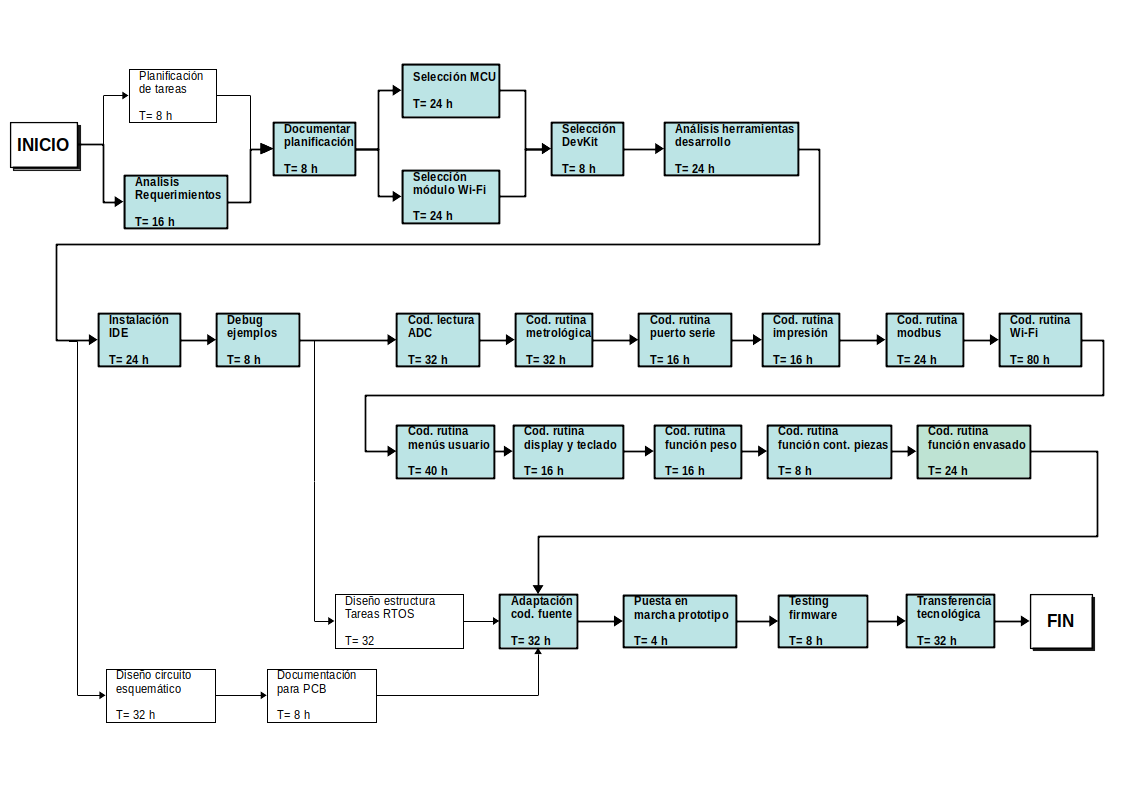
\includegraphics[width=1.15\textwidth]{./Figuras/AON.png}}
\caption{Diagrama en \textit{Activity on Node}}
\label{fig:AoN}
\end{figure}


\newpage
\section{8. Diagrama de Gantt}
\label{sec:gantt}

La Figura \ref{fig:DiagGantt} muestra el diagrama de Gantt del proyecto con la planificación inicial de ejecución de las tareas. Para esta planificación se considero la siguiente carga horaria disponible para dedicar al proyecto:
\begin{enumerate}
	\item Lunes a viernes: 2 horas diarias. 
	\item Sábados: 5 horas.
	\item Domingos: No laborables.
\end{enumerate}	
La columna \textit{work} de la figura indica la cantidad de días que conlleva cada tarea considerando la carga horaria detallada previamente y el porcentaje de dicha carga dedicada a cada tarea. Los números entre corchetes indican el porcentaje de tiempo dedicado a cada tarea que para las tareas ejecutadas en paralelo es menor a 100.
\begin{figure}[htpb]
\centering 
\rotatebox[origin=c]{0}{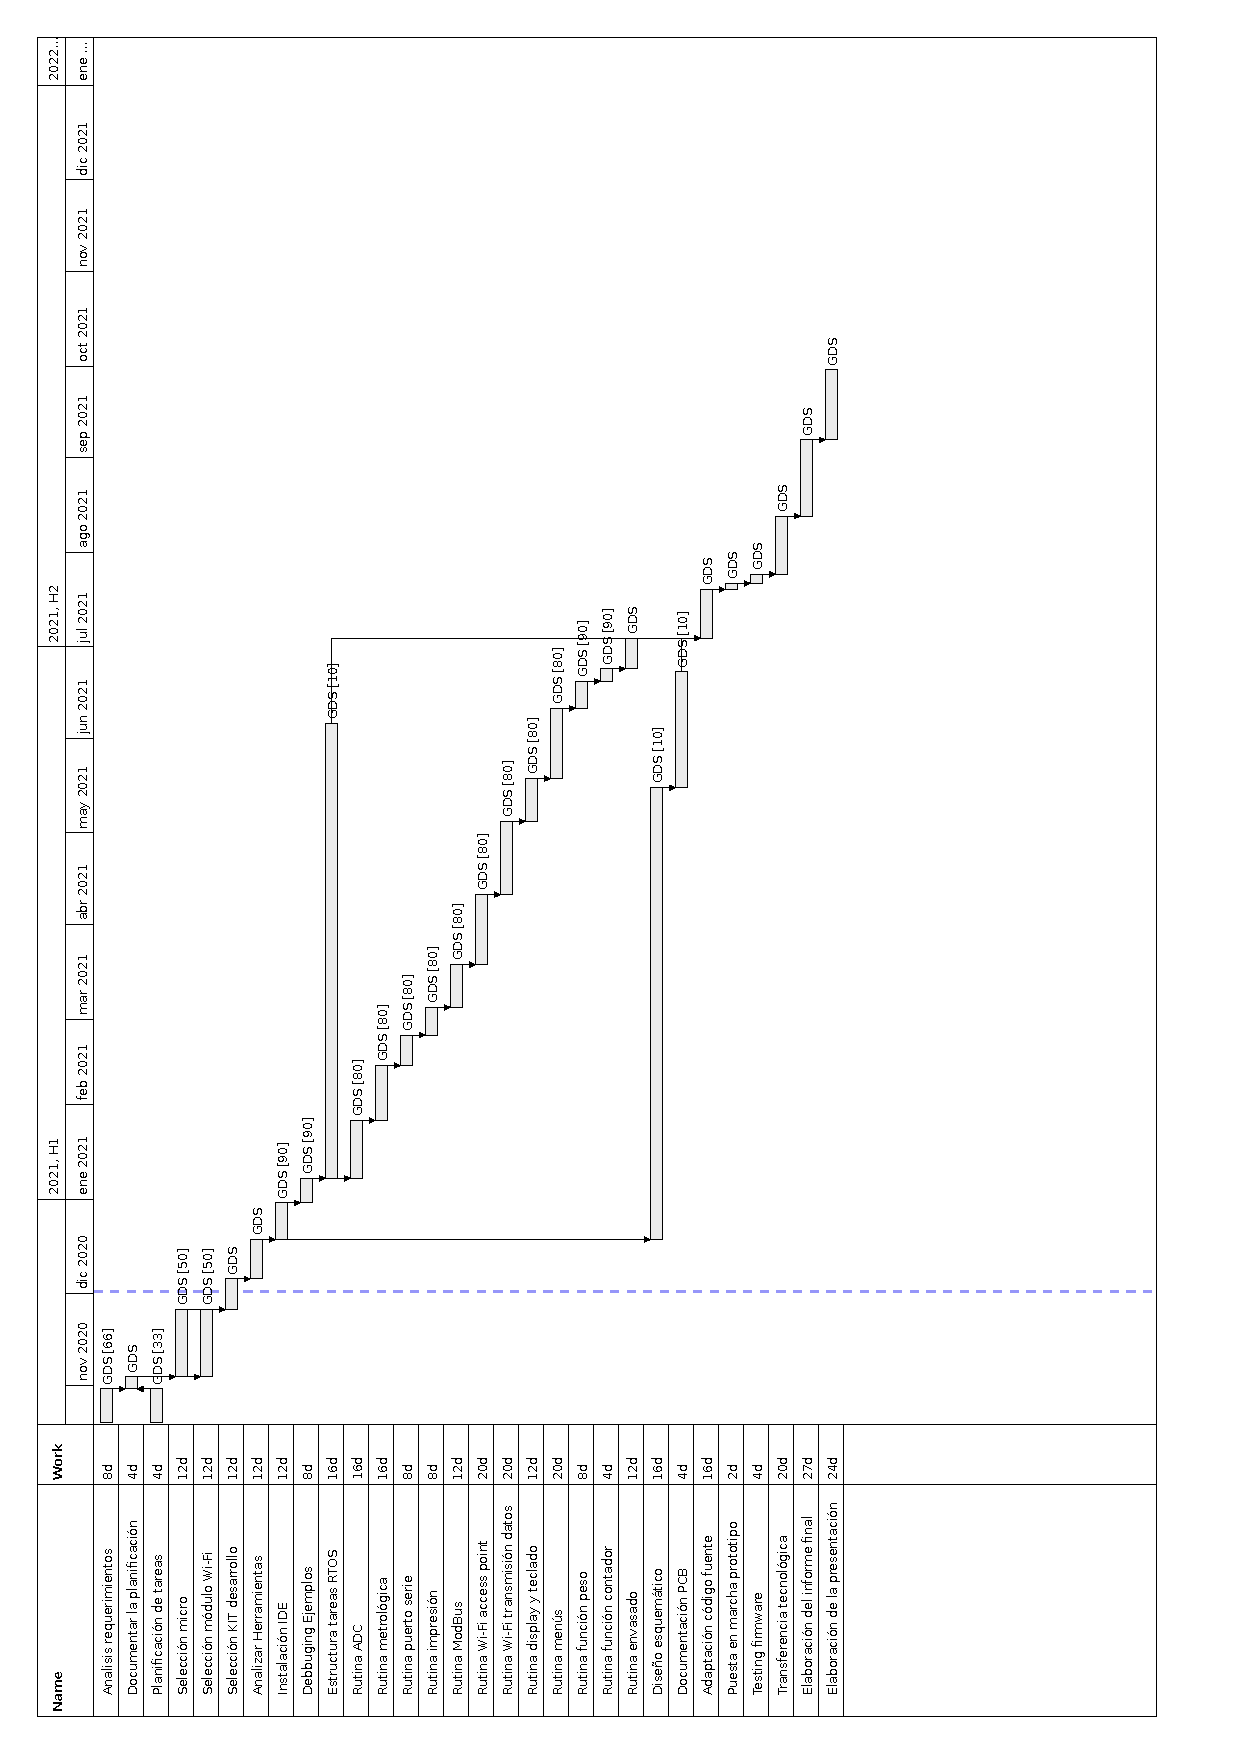
\includegraphics[width=1\textwidth]{./Figuras/gant_proyecto.pdf}}
\caption{Diagrama de gantt}
\label{fig:DiagGantt}
\end{figure}

\section{9. Matriz de uso de recursos de materiales}
\label{sec:recursos}

\begin{table}[hbt!]
\label{tab:recursos}
\centering
\begin{tabularx}{\linewidth}{@{}|c|X|X|X|X|c|@{}}
\hline
\cellcolor[HTML]{C0C0C0} & \cellcolor[HTML]{C0C0C0} & \multicolumn{4}{c|}{\cellcolor[HTML]{C0C0C0}Recursos requeridos (horas)} \\ \cline{3-6} 
\multirow{-2}{*}{\cellcolor[HTML]{C0C0C0}\begin{tabular}[c]{@{}c@{}}Código\\ WBS\end{tabular}} & \multirow{-2}{*}{\cellcolor[HTML]{C0C0C0}\begin{tabular}[c]{@{}c@{}}Nombre \\ tarea\end{tabular}} & PC & Kit desarrollo & Enrrutador Fi-Fi & Prototipo \\ \hline
1 & Análisis requerimientos					          & 16 &  &  &  \\ \hline
2 & Planificación tareas   					          &  8 &  &  &  \\ \hline
3 & Documentar la planificación				          &  8 &  &  &  \\ \hline
4 & Selección de microprocesador				          &  8 &  &  &  \\ \hline
 5 & Análisis de herramientas de desarrollo disponibles & 24 &  &  &  \\ \hline
 6 & Selección modulo comunicación Wi-Fi		          & 24 &  &  &  \\ \hline
 7 & Selección kit(s) de desarrollo                     &  8 &  &  &  \\ \hline
 8 & Instalación entorno(s) de desarrollo               & 24 &  &  &  \\ \hline 
 9 & Pruebas de compilación ejemplos y debbuging        &  8 & 8 &  &  \\ \hline
 10 & Planteo estructura tareas RTOS                    & 32 &  &  &  \\ \hline
 11 & Codificación rutinas lectura ADC                  & 32 & 32 &  &  \\ \hline
 12 & Codificación rutinas metrológicas                 & 32 & 32 &  &  \\ \hline
 13 & Codificación rutinas manejo puerto serie          & 16 & 16 &  &  \\ \hline
 14 & Codificación rutinas impresión y transmisión continua          & 16 & 16 &  &  \\ \hline

\end{tabularx}%
\end{table}

\begin{table}
\label{tab:recursos}
\centering
\begin{tabularx}{\linewidth}{@{}|c|X|X|X|X|c|@{}}
\hline
\cellcolor[HTML]{C0C0C0} & \cellcolor[HTML]{C0C0C0} & \multicolumn{4}{c|}{\cellcolor[HTML]{C0C0C0}Recursos requeridos (horas)} \\ \cline{3-6} 
\multirow{-2}{*}{\cellcolor[HTML]{C0C0C0}\begin{tabular}[c]{@{}c@{}}Código\\ WBS\end{tabular}} & \multirow{-2}{*}{\cellcolor[HTML]{C0C0C0}\begin{tabular}[c]{@{}c@{}}Nombre \\ tarea\end{tabular}} & PC & Kit desarrollo & Enrutador Wi-Fi & Prototipo \\ \hline
 15 & Codificación rutinas modbus RTU                                & 24 & 16 &  &  \\ \hline
 16 & Codificación rutinas atención de display y teclado             & 24 & 16 &  &  \\ \hline
 17 & Codificación rutinas manejo módulo Wi-Fi modo access point     & 40 & 40 & 40 &  \\ \hline
 18 & Codificación rutinas manejo módulo Wi-Fi transmisión de datos  & 40 & 40 & 40 &  \\ \hline
 19 & Codificación rutinas menús de usuario                          & 40 & 40 &  &  \\ \hline
 20 & Codificación rutinas función peso                              & 16 & 16 &  &  \\ \hline
 21 & Codificación rutinas función contador de piezas                &  8 & 16 &  &  \\ \hline
 22 & Codificación rutinas función envasado y manejo placa de potencia & 24 & 24 &  &  \\ \hline
 23 & Diseño de esquemático                                          & 32 &  &  &  \\ \hline
 24 & Documentación información para diseño PCB                      &  8 &  &  &  \\ \hline 
 25 & Adaptación código fuente                                       & 32 &  &  & 32 \\ \hline
 26 & Pruebas firmware en prototipo                                  &  8 &  & 8 & 8 \\ \hline
 27 & Redacción transferencia                                        &  40 &  &  &\\ \hline
 28 & Informe final                                                  &  64 &  &  &\\ \hline
 29 & Presentación                                                   &  24 &  &  &\\ \hline


\end{tabularx}%
\end{table}


\section{10. Presupuesto detallado del proyecto}
\label{sec:presupuesto}

%\begin{consigna}{red}
%Si el proyecto es complejo entonces separarlo en partes:
%\begin{itemize}
%\item Un total global, indicando el subtotal acumulado por cada una de las áreas.
%\item El desglose detallado del subtotal de cada una de las áreas.
%\end{itemize}
%
%IMPORTANTE: No olvidarse de considerar los COSTOS INDIRECTOS.
%
%\end{consigna}

\begin{table}[htpb]
\centering
\begin{tabularx}{\linewidth}{@{}|X|c|r|r|@{}}
\hline
\rowcolor[HTML]{C0C0C0} 
\multicolumn{4}{|c|}{\cellcolor[HTML]{C0C0C0}COSTOS DIRECTOS} \\ \hline
\rowcolor[HTML]{C0C0C0} 
Descripción &
  \multicolumn{1}{c|}{\cellcolor[HTML]{C0C0C0}Cantidad} &
  \multicolumn{1}{c|}{\cellcolor[HTML]{C0C0C0}Valor unitario} &
  \multicolumn{1}{c|}{\cellcolor[HTML]{C0C0C0}Valor total} \\ \hline
PC & 
  \multicolumn{1}{c|}{1}  &
  \multicolumn{1}{c|}{120000}  &
  \multicolumn{1}{c|}{120000} \\ \hline
Enrrutador Wi-Fi &
  \multicolumn{1}{c|}{1} &
  \multicolumn{1}{c|}{4000} &
  \multicolumn{1}{c|}{4000} \\ \hline
Kit desarrollo &
  \multicolumn{1}{c|}{1} &
  \multicolumn{1}{c|}{8000} &
  \multicolumn{1}{c|}{8000} \\ \hline
Horas hombre Ingeniería &
  \multicolumn{1}{c|}{670} &
  \multicolumn{1}{c|}{1000} &
  \multicolumn{1}{c|}{670000} \\ \hline
      
\multicolumn{1}{|l|}{} &
   &
   &
   \\ \hline
\multicolumn{3}{|c|}{SUBTOTAL}  &
  \multicolumn{1}{c|}{802000} \\ \hline
\rowcolor[HTML]{C0C0C0} 
\multicolumn{4}{|c|}{\cellcolor[HTML]{C0C0C0}COSTOS INDIRECTOS} \\ \hline
\rowcolor[HTML]{C0C0C0} 
Descripción &
  \multicolumn{1}{c|}{\cellcolor[HTML]{C0C0C0}Cantidad} &
  \multicolumn{1}{c|}{\cellcolor[HTML]{C0C0C0}Valor unitario} &
  \multicolumn{1}{c|}{\cellcolor[HTML]{C0C0C0}Valor total} \\ \hline
Servicio de internet & 
  \multicolumn{1}{c|}{12}  &
  \multicolumn{1}{c|}{2000}  &
  \multicolumn{1}{c|}{24000} \\ \hline  
\multicolumn{1}{|l|}{} &
   &
   &
   \\ \hline
\multicolumn{3}{|c|}{SUBTOTAL} &
  \multicolumn{1}{c|}{24000} \\ \hline
\rowcolor[HTML]{C0C0C0}
\multicolumn{3}{|c|}{TOTAL} &
   826000 \\ \hline
\end{tabularx}%
\end{table}


\section{11. Matriz de asignación de responsabilidades}
\label{sec:responsabilidades}

%\begin{consigna}{red}
%Establecer la matriz de asignación de responsabilidades y el manejo de la autoridad completando la siguiente tabla:

\begin{table}[htpb]
\centering
\resizebox{\textwidth}{!}{%
\begin{tabular}{|c|c|c|c|c|c|}
\hline
\rowcolor[HTML]{C0C0C0} 
\cellcolor[HTML]{C0C0C0} &
  \cellcolor[HTML]{C0C0C0} &
  \multicolumn{4}{c|}{\cellcolor[HTML]{C0C0C0}Listar todos los nombres y roles del proyecto} \\ \cline{3-6} 
\rowcolor[HTML]{C0C0C0} 
\cellcolor[HTML]{C0C0C0} &
  \cellcolor[HTML]{C0C0C0} &
  Responsable &
  Orientador &
  Equipo &
  Cliente \\ \cline{3-6} 
\rowcolor[HTML]{C0C0C0} 
\multirow{-3}{*}{\cellcolor[HTML]{C0C0C0}\begin{tabular}[c]{@{}c@{}}Código\\ WBS\end{tabular}} &
  \multirow{-3}{*}{\cellcolor[HTML]{C0C0C0}Nombre de la tarea} &
  \authorname &
  \supname &
  N/A &
  \clientename \\ \hline
  
1 & Análisis requerimientos					         & P &  &  & A  \\ \hline
2 & Planificación tareas   					         & P & I&  &  \\ \hline
3 & Documentar la planificación				         & P & A-C&  & A \\ \hline
4 & Selección de microprocesador				         & P & A&  &  \\ \hline
5 & Análisis de herramientas de desarrollo disponibles & P & A&  &  \\ \hline 
6 & Selección modulo comunicación Wi-Fi		         & P & A&  &  \\ \hline
7 & Selección kit(s) de desarrollo                     & P & I&  &  \\ \hline
8 & Instalación entorno(s) de desarrollo               & P &  &  &  \\ \hline 
9 & Pruebas de compilación ejemplos y debbuging        & P &  &  &  \\ \hline
10 & Planteo estructura tareas RTOS                    & P &  &  &  \\ \hline
11 & Codificación rutinas lectura ADC                  & P & C&  &  \\ \hline
12 & Codificación rutinas metrológicas                 & P & C&  &  \\ \hline
13 & Codificación rutinas manejo puerto serie          & P &  &  &  \\ \hline
14 & Codificación rutinas impresión y transmisión continua          & P &  &  &  \\
15 & Codificación rutinas modbus RTU                                & P & C&  &  \\ \hline
16 & Codificación rutinas atención de display y teclado             & P &  &  &  \\ \hline
17 & Codificación rutinas manejo módulo Wi-Fi modo access point     & P &  &  &  \\ \hline
18 & Codificación rutinas manejo módulo Wi-Fi transmisión de datos  & P &  &  &  \\ \hline
19 & Codificación rutinas menús de usuario                          & P & C&  &  \\ \hline
20 & Codificación rutinas función peso                              & P & C&  &  \\ \hline
21 & Codificación rutinas función contador de piezas                & P & C&  &  \\ \hline
22 & Codificación rutinas función envasado y manejo placa de potencia & P & C &  &  \\ \hline
23 & Diseño de esquemático                                          & P & A-C &  &  \\ \hline
24 & Documentación información adicional para diseño PCB            & P & A &  &  \\ \hline 
25 & Adaptación código fuente                                       & P &  &  &  \\ \hline
26 & Pruebas firmware en prototipo                                  & P & A &  & A \\ \hline
27 & Redacción transferencia                                        & P & A &  & A \\ \hline 

\end{tabular}%
}
\end{table}

{\footnotesize
Referencias:
\begin{itemize}
	\item P = Responsabilidad Primaria
	\item S = Responsabilidad Secundaria
	\item A = Aprobación
	\item I = Informado
	\item C = Consultado
\end{itemize}
} %footnotesize

%Una de las columnas debe ser para el Director, ya que se supone que participará en el proyecto.
%A su vez se debe cuidar que no queden muchas tareas seguidas sin ``A'' o ``I''.
%
%Importante: es redundante poner ``I/A'' o ``I/C'', porque para aprobarlo o responder consultas primero la persona debe ser informada.
%
%\end{consigna}

\section{12. Gestión de riesgos}
\label{sec:riesgos}

%\begin{consigna}{red}
%a) Identificación de los riesgos (al menos cinco) y estimación de sus consecuencias:
% 
%Riesgo 1: detallar el riesgo (riesgo es algo que si ocurre altera los planes previstos)
%\begin{itemize}
%\item Severidad (S): mientras más severo, más alto es el número (usar números del 1 al 10).\\
%Justificar el motivo por el cual se asigna determinado número de severidad (S).
%\item Probabilidad de ocurrencia (O): mientras más probable, más alto es el número (usar del 1 al 10).\\
%Justificar el motivo por el cual se asigna determinado número de (O). 
%\end{itemize}   
%
%Riesgo 2:
%\begin{itemize}
%\item Severidad (S): 
%\item Ocurrencia (O):
%\end{itemize}
%
%Riesgo 3:
%\begin{itemize}
%\item Severidad (S): 
%\item Ocurrencia (O):
%\end{itemize}


%b) Tabla de gestión de riesgos:      (El RPN se calcula como RPN=SxO)

\begin{table}[H]% [!htpb]
\centering
\begin{tabularx}{\linewidth}{@{}|X|c|c|c|c|c|c|@{}}
\hline
\rowcolor[HTML]{C0C0C0} 
Riesgo & S & O & RPN & S* & O* & RPN* \\ \hline

Objeciones realizadas por el organismo regulador a funcionalidades del software que impliquen la no aprobación del expediente del producto. La ley metrológica Argentina es obsoleta y no contempla muchas de las características de los equipos actuales. Esto genera ambigüedades en los requerimientos para la aprobación de un nuevo instrumento quedando su resolución a criterio del organismo regulador. Es habitual que durante el proceso de aprobación estas objeciones impliquen cambios en el firmware.    
& 3 & 8 & 24 & &  & \\ \hline

Fallas de diseño de circuito que impliquen susceptibilidad al ruido eléctrico o deriva térmica con el consiguiente riesgo de no superar los ensayos metrológicos de aprobación de modelo. La aprobación de un nuevo modelo implica aprobar ensayos de inmunidad electromagnética y ensayos metrológicos (movilidad, excentricidad, repetitividad, etc) realizados en una cámara térmica en todo el rango de temperatura de operación declarado en el expediente. La necesidad de instalaciones especiales y alto de costo de tercerizar estos ensayos los vuelven inviables de ser realizados durante el proceso de diseño.       
& 9 & 4 & 36 &  9  &  2  & 18     \\ \hline

Obsolescencia de componentes críticos como ser el procesador, el ADC, controlador de display etc. Es común que los fabricantes de semiconductores descontinúen la fabricación de componentes o de ciertos encapsulados de un componente. También es habitual que exista una gran oferta por parte de los distribuidores cuando los componentes están próximos a ser discontinuados incluso en ocasiones a menor precio que el habitual volviéndolos falsamente atractivos durante el proceso de selección.       
& 9  & 5  & 45 &  9  &  1  & 9     \\ \hline

Demoras en la fabricación de la placa del prototipo con el consiguiente retraso de todas las etapas que dependan de contar con un prototipo físico para ser ejecutadas. Principalmente se retrasará la validación del diseño que debe hacerse sobre el producto final y por ende se podría retrasar la puesta producción. Las demoras en la fabricación de un prototipo habitualmente suelen estar asociadas a que son procesos que se ejecutan por fuera de los procesos estándares de las empresas lo cual lo vuelve mas propenso a imprevistos. Un ejemplo es el tener que comprar componentes que no se encuentran dentro del sistema de stock de la compañía. 
& 3  & 5  & 15 &    &    &      \\ \hline

Errores al documentar los requerimientos del proyecto que puedan implicar que no se implementen funcionalidades requeridas o que se implementen incorrectamente. Puede ocurrir por mala comunicación entre las partes involucradas o porque alguna de las partes supone que cierto requerimiento se sobreentiende y no es necesario aclararlo y/o documentarlo
& 8 & 8 & 56 & 4   &  4  &  16    \\ \hline
       
\end{tabularx}
\end{table}

Criterio adoptado: 
Se tomarán medidas de mitigación en los riesgos cuyos números de RPN sean mayores a 25.

Nota: los valores marcados con (*) en la tabla corresponden luego de haber aplicado la mitigación.

Plan de mitigación de los riesgos que originalmente excedían el RPN máximo establecido:
 
Riesgo 1: N/A. Las correcciones a realizar suelen ser pequeñas con bajo costo de rediseño.
%plan de mitigación (si por el RPN fuera necesario elaborar un plan de mitigación).
%  Nueva asignación de S y O, con su respectiva justificación:
%  - Severidad (S): mientras más severo, más alto es el número (usar números del 1 al 10).
%          Justificar el motivo por el cual se asigna determinado número de severidad (S).
%  - Probabilidad de ocurrencia (O): mientras más probable, más alto es el número (usar del 1 al 10).
%          Justificar el motivo por el cual se asigna determinado número de (O).

Riesgo 2: Para las partes del circuito que sean propensas a generar deriva térmica de la lectura se procurará seleccionar componentes de baja dispersión y rango de temperatura de trabajo igual o mayor al rango de temperatura de uso del equipo. También se consultarán las notas de aplicación provistas por el fabricante del ADC para una correcta selección de componentes y especialmente se tomarán como referencia diseños previos de comprobado desempeño.\\ 
En lo respectivo a la susceptibilidad electromagnética se procurará atenerse a las buenas prácticas de diseños de PCB con mayor atención en el diseño del stack del PCB, el trazado de las pistas de potencia y la ubicación de los componentes radiantes respecto del circuito de medición. Para el stack del PCB se utilizará un modelo de 4 capas con planos internos de GND y Vcc que generen caminos de retornos de las corrientes bien definidos. Para los elementos radiantes (bobinas de fuentes switching o módulo wi-fi) se seguirán cuidadosamente las recomendaciones de los fabricantes de componentes sobre el trazado de pistas y ubicación de los mismos.\\
Nueva posibilidad de ocurrencia = 2. 
 
Riesgo 3: Para los componentes críticos se seleccionarán unicamente aquellos componentes cuyos fabricantes aseguren una longevidad no menor a 6 años y preferentemente aquellos que aseguren 10 o mas años de longevidad.\\
Nueva posibilidad de ocurrencia = 1. 

Riesgo 4: N/A. Las demoras de este tipo usualmente pueden quedar enmascaradas en variaciones de tiempo de ejecución del proyecto.

Riesgo 5: Se revisarán los requerimientos registrados con todas las partes involucradas (área comercial, gerencia, área ingeniería) confirmando que no se haya omitido algún item. También se realizarán entregas parciales o demostraciones parciales durante el proceso de desarrollo para confirmar que las funcionalidades implementadas cumplan lo pretendido. De esta manera se minimiza la posibilidad de ocurrencia de malas interpretaciones. Por otro lado, de haber diferencias entre lo pretendido y lo implementado estas discrepancias deberían ser menores minimizando la severidad del problema.\\
Nueva posibilidad de ocurrencia = 4\\
Nueva severidad = 4
%\end{consigna}


\section{13. Gestión de la calidad}
\label{sec:calidad}

%\begin{consigna}{red}
%Para cada uno de los requerimientos del proyecto indique:
%\begin{itemize} 
%\item Req \#1: copiar acá el requerimiento.
%
%Verificación y validación:
%
%\begin{itemize}
%\item Verificación para confirmar si se cumplió con lo requerido antes de mostrar el sistema al cliente. Detallar 
%\item Validación con el cliente para confirmar que está de acuerdo en que se cumplió con lo requerido. Detallar  
%\end{itemize}
%
%\end{itemize}
%
%Tener en cuenta que en este contexto se pueden mencionar simulaciones, cálculos, revisión de hojas de datos, consulta con expertos, mediciones, etc.
%
%\begin{itemize}
%\item Verificación: 
%\item Validación:
%\end{itemize}	
%
%\end{consigna}

\begin{enumerate}
\item Costo
	\begin{enumerate}
	\item El producto (placa electrónica con display) deberá tener un costo menor o igual a U\$S 30. %
	\end{enumerate}
	
\begin{itemize}
\item Verificación: Cotización de todos los componentes y procesos de producción.
\item Validación:El costo de producción del prototipo puede servir de validación. En caso de que el costo resultante dependa sensiblemente de las cantidades producidas se validará con la producción de la primer tanda.
\end{itemize}
	
\item Interfaz de usuario y conectividad
	\begin{enumerate}
	\item Teclado con 5 teclas multifunción cuyas funciones son Encendido/Apagado, puesta a cero, toma de tara, imprimir ticket, ingreso a menú, navegación.
	
\begin{itemize}
\item Verificación:corroborando que el código fuente implementa las funciones indicadas para cada tecla.
\item Validación: con demostraciones de funcionamiento en entregas parciales del código.
\end{itemize}
	
	\item Display LCD con 6 dígitos, indicador de nivel de batería, indicadores metrológicos (centro de cero, movimiento y tara tomada) e indicador de unidad de peso. Se deberá reutilizar el display utilizado actualmente en el equipo NEO.

\begin{itemize}
\item Verificación: corroborando que el código fuente maneja todos los indicadores del display según  lo requerido.
\item Validación: con demostraciones de funcionamiento en entregas parciales del código.
\end{itemize}	
	
	\item Un puerto serie con interfaz RS232/RS485 seleccionable via jumpers, Baudrate configurable y lineas de handshake opcionales. El puerto serie podrá funcionar en las modalidades de transmisión continua del peso en formato ASCII con formato configurable, protocolo ModBus RTU esclavo, impresión de ticket para conexión a impresora de 32 lineas con formato configurable. 
	
\begin{itemize}
\item Verificación: Simulaciones de uso trasmitiendo datos a un programas tipo terminal e intercambiando datos con programas de simulación de Modbus (ejemplo Modscan).
\item Validación: demostraciones de uso conectando el equipo a impresoras térmicas, dispositivos modbus y capturando el envío continuo de datos con alguno de los software de la compañía.
\end{itemize}		
	
	\item Conexión Wi-Fi con antena interna o externa según sea para gabinetes metálicos o plásticos. El módulo Wi-Fi podrá funcionar en modo access point que permitirá conectarse desde otro dispositivo para configurar parámetros de acceso a la red Wi-Fi y en modo cliente para el resto de las funciones.
	
\begin{itemize}
\item Verificación: conectado la PC al access point y abriendo la comunicación con un software terminal. En modo cliente abriendo la comunicación desde un programa terminal al IP asignado dentro de la red.
\item Validación: Se pueden hacer demostraciones con los mismos métodos utilizados en la verificación.
\end{itemize}		
	
	\item Manejo vía bus I2C de placa auxiliar de entradas/salidas de potencia.
	\end{enumerate}
	
\begin{itemize}
\item Verificación: con funciones de debug que permitan leer y escribir los puertos de la placa de potencia. Las placas de potencia poseen LEDs que evidencian el estado de sus puertos no precisando otro hardware externo para estas pruebas. El cliente proveerá una placa de potencia para utilizar durante el desarrollo.
\item Validación: Se validará junto con la demostración de los modos de automatismo detallados mas adelante.
\end{itemize}		
	
\item Fuente de energía
	\begin{enumerate}
	\item El equipo se alimentará desde una fuente externa de 12Vcc.
	
\begin{itemize}
\item Verificación: mediante la revisión del diseño de las etapas de las fuentes de alimentación
\item Validación: Alimentando el prototipo con la fuente externa prevista para ser utilizada con el equipo.
\end{itemize}		
	
	\item Opcionalmente el equipo podrá contar con una batería interna con capacidad para uso continuo de 8 horas.
	\item Durante el diseño del circuito esquemático se hará una evaluación de costos para definir si el circuito de control de carga de la batería se implementa dentro de la placa principal del equipo base o como una placa satélite opcional.
		\item No se implementará en el código fuente las funcionalidades de modo batería (nivel de batería, apagado automático de display, etc) debiendo implementarse en futuras revisiones a cargo de la empresa. 
	
\begin{itemize}
\item Verificación: verificando los costos con cotizaciones parciales durante el desarrollo y revisando los cálculos de consumo y diseño de la etapa de carga de batería.
\item Validación: Con ensayos de autonomía de uso del prototipo alimentado con la batería.
\end{itemize}	
	\end{enumerate}

\item Ajustes metrológicos
	\begin{enumerate}
	\item El equipo debe ser de clase III pudiendo manejar hasta 10.000 (diez mil) divisiones de display.
	
\begin{itemize}
\item Verificación: con funciones de debug que simulen la lectura de peso.
\item Validación: mediante demostraciones de entregas parciales y durante los ensayos metrológico realizados al prototipo ya sea con un simulador de carga o conectado a un receptor de carga y peso patrones.
\end{itemize}		
	
	\item El acceso al menú de ajuste metrológicos debe estar protegido con un jumper interno que requiera la rotura de un precinto legal para ser accedido.
	
\begin{itemize}
\item Verificación: simulando el ingreso al menú con y sin el jumper colocado.
\item Validación: mediante demostraciones de entregas parciales y durante procesos de ajuste realizados sobre el prototipo previo a la realización de ensayos metrológicos.
\end{itemize}			
	 
	\item El menú de ajustes metrológicos debe permitir seleccionar la capacidad máxima del indicador, el incremento y el la cantidad de posiciones decimales. Si la elección de capacidad e incremento es tal que se superen las 10.000 divisiones el equipo debe dar señal de error.
	
\begin{itemize}
\item Verificación: simulando el ajuste del equipo con diversas combinaciones de capacidad e incremento.
\item Validación: mediante demostraciones de entregas parciales y durante procesos de ajuste realizados sobre el prototipo previo a la realización de ensayos metrológicos.
\end{itemize}		
	
	\item Este menú también debe permitir realizar las acciones de toma de cero de calibración y ajuste con peso patrón en hasta 3 puntos.
	
\begin{itemize}
\item Verificación: con funciones de debug que simulen la lectura de peso y simulando el ajuste del equipo con 1, 2 y tres puntos de peso patrón.
\item Validación: mediante demostraciones de entregas parciales y durante el proceso de ajuste realizados sobre el prototipo previo a la realización de ensayos metrológicos.
\end{itemize}		
	
	\end{enumerate}
\item Almacenamiento de información
	\begin{enumerate}
	\item El equipo debe contar con una memoria no volátil para almacenar los parámetros de ajustes metrológicos, parámetros de configuración y totalizadores. 
	\item Todos los datos almacenados en dicha memoria deben estar protegidos con un CRC que garantice su integridad al ser recuperados. Si los valores de ajuste metrológicos se vieran comprometidos el equipo debe dar señal de error impidiendo su uso normal.
	\item Es de preferencia el uso de memorias de tecnología ferromagnética por sus casi infinitos ciclos de escritura. 
	
\begin{itemize}
\item Verificación: mediante funciones de debug que permitan recuperar los datos almacenados en la memoria y que permitan simular errores de CRC.
\item Validación: mediante demostraciones de entregas parciales  donde apagando y encendiendo el prototipo se corrobore que los parámetros de ajuste y configuración se mantuvieron inalterados. También imprimiendo tiques con el resumen de los totalizadores y verificando que coincidan con las capturas de peso que se hayan hecho durante las demostraciones.
\end{itemize}		
	\end{enumerate}	
	
\item Celdas de carga
	\begin{enumerate}
	\item El equipo debe admitir celdas de carga con relaciones excitación/señal de 1 mV/V, 2 mV/V y 3 mV/V.
	\item Debe contar con una fuente de tensión regulada de 5V con baja deriva térmica exclusiva para la excitación de las celdas de carga.
	\item Debe poder excitar hasta 12 celdas conectadas en paralelo de 750ohms cada una sin variaciones en su tensión de salida. 
	\item Debe contar con una segunda salida de excitación regulada con un preset que permita la conexión y ecualización de dos celdas de carga. Para mas de dos celdas la ecualización se debe realizar mediante una caja de unión externa.
	\item Para la lectura de la señal de salida de las celdas se deberá utilizar el ADC \textit{ADS1232} ya utilizado en otros diseños de la compañía por sus ya comprobadas prestaciones.
	
\begin{itemize}
\item Verificación: Todos los requisitos para la conexión y uso de celdas de carga se verificarán mediante la revisión del diseño electrónico y los cálculos de componentes respectivos. 
\item Validación: La conexión y uso de las celdas de carga se validará ensayando el prototipo conectado a diversos receptores de carga cada uno con distintos tipos y cantidades de celdas o en su defecto con simuladores de carga.
\end{itemize}		
	
	\end{enumerate}	
\item El equipo debe implementar las siguientes funciones:
	\begin{enumerate}
	\item Peso (función por defecto).
	\item Contador de piezas.
	\item Envasado con doble corte (requiere placa auxiliar de potencia).
	\item El código fuente se debe estructurar de manera tal que permita en un futuro agregar funciones de forma estructurada y sencilla.
	
\begin{itemize}
\item Verificación: los modos funciones se verificarán simulando el uso de cada una de ellas y de cada una de las funcionalidades asociadas. En el caso que alguna función o funcionalidad requiera el uso de alguna pieza de hardware de la cual no se disponga se hará uso de funciones de debug que simulen dicho hardware.
\item Validación: Todas las funciones se validarán haciendo ensayos de uso del prototipo realizados por personal de ingeniería involucrado en el proyecto y por personal técnico de la empresa ajeno al proyecto.
\end{itemize}		
	
	\end{enumerate}				
\end{enumerate}

\section{14. Comunicación del proyecto}
\label{sec:comunicaciones}

El plan de comunicación del proyecto es el siguiente:

\begin{table}[htpb]
\centering
\begin{tabularx}{\linewidth}{@{}|X|C{2.4cm}|C{3cm}|C{1.8cm}|C{2cm}|C{2.1cm}|@{}}
\hline
\rowcolor[HTML]{C0C0C0} 
\multicolumn{6}{|c|}{\cellcolor[HTML]{C0C0C0}PLAN DE COMUNICACIÓN DEL PROYECTO}           \\ \hline
\rowcolor[HTML]{C0C0C0} 
¿Qué comunicar? & Audiencia & Propósito & Frecuencia & Método de comunicac. & Responsable \\ \hline

Avances en la selección de componentes o en el diseño del circuito esquemático & 
Jefe de ingeniería  &  
validar requisitos de hardware y/o consensuar cambios en los mismos de ser necesario  &  
cada 15 días   & 
video llamada  &     
Sanchez Gonzalo        \\ \hline

Finalización del circuito esquemático  & 
Equipo de electrónica del depto de ingeniería &
Hacer un cierre de la etapa y fijar pautas para el diseño del PCB y fabricación de la placa prototipo   por parte de la empresa&
Por única vez  &
video llamada & 
Sanchez Gonzalo            \\ \hline

Avances en el desarrollo del código fuente & 
Jefe de ingeniería  &  
Realizar demostraciones y validaciones parciales de los requisitos de software y/o consensuar cambios en los mismos de ser necesario  &  
cada 15 días   & 
video llamada  &     
Sanchez Gonzalo        \\ \hline

Finalización del firmware  & 
Equipo de electrónica del depto de ingeniería &
Hacer un cierre de la etapa y fijar pautas para la realización de ensayos con la versión final del firmware sobre la placa prototipo&
Por única vez  &
video llamada & 
Sanchez Gonzalo   \\ \hline

\end{tabularx}
\end{table}


\begin{table}[htpb]
\centering
\begin{tabularx}{\linewidth}{@{}|X|C{2.4cm}|C{3cm}|C{1.8cm}|C{2cm}|C{2.1cm}|@{}}
\hline
\rowcolor[HTML]{C0C0C0} 
\multicolumn{6}{|c|}{\cellcolor[HTML]{C0C0C0}PLAN DE COMUNICACIÓN DEL PROYECTO (continuación)}           \\ \hline
\rowcolor[HTML]{C0C0C0} 
¿Qué comunicar? & Audiencia & Propósito & Frecuencia & Método de comunicac. & Responsable \\ \hline

Entrega de transferencia tecnológica  &
Departamento de ingeniería y gerencia   &
Presentación del prototipo, demostraciones y cierre formal del proyecto  &
Por única vez  &
A consensuar. Podrá presencial o semi presencial dependiendo de las condiciones sanitarias públicas al momento del cierre del proyecto   & 
Sanchez Gonzalo            \\ \hline
\end{tabularx}
\end{table}



\section{15. Gestión de compras}
\label{sec:compras}

Dpto. compras Sipel S.R.L., \\
Se solicita la adquisición de un kit de desarrollo marca Spressif modelo ESP-WROVER-KIT-VE. Realizar la adquisición 	mediante compra en linea en los distribuidores www.mouser.com o www.digikey.com.	Realizar la importación mediante servicio de currier cuyo tiempo promedio de entrega es de 15 dias corridos. No se debe consolidar la compra del kit con otros productos para evitar demoras en la gestión de compras, envío o en el ingreso aduanero.
En el distribuidor Mouser el producto está codificado como 356-ESPWROVER-KIT-VB. En el distribuidor Digikey el producto está codificado como 1904-1013-ND.

Saludos atte.,\\
Ing. Sanchez Gonzalo.
%\begin{consigna}{red}
%En caso de tener que comprar elementos o contratar servicios:
%a) Explique con qué criterios elegiría a un proveedor.
%b) Redacte el Statement of Work correspondiente.
%\end{consigna}

\section{16. Seguimiento y control}
\label{sec:seguimiento}

%\begin{consigna}{red}
%Para cada tarea del proyecto establecer la frecuencia y los indicadores con los se seguirá su avance y quién será el responsable de hacer dicho seguimiento y a quién debe comunicarse la situación (en concordancia con el Plan de Comunicación del proyecto).
%
%El indicador de avance tiene que ser algo medible, mejor incluso si se puede medir en \% de avance. Por ejemplo,se pueden indicar en esta columna cosas como ``cantidad de conexiones ruteadeas'' o ``cantidad de funciones implementadas'', pero no algo genérico y ambiguo como ``\%'', porque el lector no sabe porcentaje de qué cosa.
%
%\end{consigna}

\begin{longtable}{|m{1cm}|m{3.5cm}|m{2.2cm}|m{2cm}|m{3cm}|m{1.5cm}|}
\hline
\rowcolor[HTML]{C0C0C0} 
\multicolumn{6}{|c|}{\cellcolor[HTML]{C0C0C0}SEGUIMIENTO DE AVANCE}                                                                       \\ \hline
\rowcolor[HTML]{C0C0C0} 
Tarea del WBS 			& Indicador de avance & Frecuencia de reporte & Resp. de seguimiento & Persona a ser informada & Método de comunic. \\ \hline
\endfirsthead

\hline
\rowcolor[HTML]{C0C0C0} 
\multicolumn{6}{c}{\cellcolor[HTML]{C0C0C0}SEGUIMIENTO DE AVANCE}                                                                       \\ \hline
\rowcolor[HTML]{C0C0C0} 
Tarea del WBS 			& Indicador de avance & Frecuencia de reporte & Resp. de seguimiento & Persona a ser informada & Método de comunic. \\ \hline
\endhead

\multicolumn{6}{c}{Continúa}
\endfoot

\endlastfoot

1.1	& Fecha de inicio  & Única vez al comienzo & \authorname & \clientename, \supname & email \\ \hline
2.1	& Avance de las subtareas  & Mensual mientras dure la tarea & \authorname & \clientename, \supname & email \\ \hline

\end{longtable}

\begin{table}[!htpb]
\centering
%\begin{tabularx}{\linewidth}{@{}|X|X|X|X|X|X|@{}}
\begin{tabularx}{\linewidth}{@{}|X|C{2.5cm}|C{3cm}|C{2cm}|C{2cm}|C{2.5cm}|@{}}
\hline
\rowcolor[HTML]{C0C0C0} 
\multicolumn{6}{|c|}{\cellcolor[HTML]{C0C0C0}SEGUIMIENTO DE AVANCE}                                                                       \\ \hline
\rowcolor[HTML]{C0C0C0} 
Tarea del WBS & Indicador de avance & Frecuencia de reporte & Resp. de seguimiento & Persona a ser informada & Método de comunic. \\ \hline

%tarea
1 &
%indicador avance 
Plan de trabajo  &  
%frecuencia  
Única vez  &  
%responsable  
Sanchez Gonzalo  &  
%a quien se informa  
Director del proyecto y Cliente  &
%metodo  
email    \\ \hline
 
%tarea
2 &
%indicador avance 
Tabla comparativa con prestaciones vs. costo de microprocesadores y módulos Wi-Fi preseleccionados.  &  
%frecuencia  
semanal  &  
%responsable  
Sanchez Gonzalo  &  
%a quien se informa  
Director de proyecto  &
%metodo  
Documento en linea compartido y video llamada    \\ \hline
    
%tarea
3 &
%indicador avance 
entregas parciales de código y demostraciones de módulos implementados  &  
%frecuencia  
quincenal  &  
%responsable  
Sanchez Gonzalo  &  
%a quien se informa  
Director de proyecto  &
%metodo  
repositorio GIT para la entrega de código y video llamadas para las demostraciones.    \\ \hline
    
%tarea
4 &
%indicador avance 
Entregas parciales de esquemáticos en formato PDF y entrega final de esquemáticos como proyecto de Altium. Actualizaciones de lista de materiales y documentos con pautas para diseño del PCB  &  
%frecuencia  
Mensual  &  
%responsable  
Sanchez Gonzalo  &  
%a quien se informa  
Director de proyecto  &
%metodo  
Los archivos esquemáticos se compartirán vía Google Drive mientras que las listas de materiales y pautas para diseño de PCB serán respectivamente hojas de datos y documentos de textos compartidos online.   \\ \hline

%tarea
5 &
%indicador avance 
entregas parciales de código y demostración de funcionalidades sobre prototipo   &  
%frecuencia  
semanal  &  
%responsable  
Sanchez Gonzalo  &  
%a quien se informa  
Director de proyecto  &
%metodo  
repositorio GIT para la entrega de código y video llamadas para las demostraciones.    \\ \hline

\end{tabularx}%
%}
\end{table}

\begin{table}[!htpb]
\centering
%\begin{tabularx}{\linewidth}{@{}|X|X|X|X|X|X|@{}}
\begin{tabularx}{\linewidth}{@{}|X|C{2.5cm}|C{3cm}|C{2cm}|C{2cm}|C{2.5cm}|@{}}
\hline
\rowcolor[HTML]{C0C0C0} 
\multicolumn{6}{|c|}{\cellcolor[HTML]{C0C0C0}SEGUIMIENTO DE AVANCE(continuación)}                                                                       \\ \hline
\rowcolor[HTML]{C0C0C0} 
Tarea del WBS & Indicador de avance & Frecuencia de reporte & Resp. de seguimiento & Persona a ser informada & Método de comunic. \\ \hline
    
%tarea
6 &
%indicador avance 
Entregas parciales de documentación  &  
%frecuencia  
quincenal  &  
%responsable  
Sanchez Gonzalo  &  
%a quien se informa  
Director proyecto y cliente  &
%metodo  
Documentos compartidos vía Google Drive    \\ \hline
    
%tarea
7 &
%indicador avance 
Entregas parciales de informe final y presentación para correcciones  &  
%frecuencia  
Semanal  &  
%responsable  
Sanchez Gonzalo  &  
%a quien se informa  
  &
%metodo  
Documentos compartido vía Google Drive    \\ \hline
    

\end{tabularx}%
%}
\end{table}

\section{17. Procesos de cierre}    
\label{sec:cierre}

%\begin{consigna}{red}
%Establecer las pautas de trabajo para realizar una reunión final de evaluación del proyecto, tal que contemple las siguientes actividades:
%
%\begin{itemize}
%\item Pautas de trabajo que se seguirán para analizar si se respetó el Plan de Proyecto original:
% - Indicar quién se ocupará de hacer esto y cuál será el procedimiento a aplicar. 
%\item Identificación de las técnicas y procedimientos útiles e inútiles que se utilizaron, y los problemas que surgieron y cómo se solucionaron:
% - Indicar quién se ocupará de hacer esto y cuál será el procedimiento para dejar registro.
%\item Indicar quién organizará el acto de agradecimiento a todos los interesados, y en especial al equipo de trabajo y colaboradores:
%  - Indicar esto y quién financiará los gastos correspondientes.
%\end{itemize}
%
%\end{consigna}

Pautas de trabajo que se seguirán para analizar si se respetó el Plan de Proyecto original:
\begin{itemize}
\item Encargado: Gonzalo Daniel Sanchez.
\item Al concluir el proyecto se realizará una reunión final del proyecto con los integrantes del área de ingeniería de Sipel SRL, el jefe del área Ezequiel Marengo, el jefe del área comercial Daniel Pluss y el gerente general de la firma Iván Brenboim. 
\item En esta reunión se evaluará el cumplimiento del Plan de Proyecto original contrastando las fechas y carga horaria planificadas para la ejecución de las distintas etapas y las respectivas fechas y horas reales. También serán analizados los requerimientos originales y comparados con el prototipo presentado y así
determinar el grado de objetivos cumplidos.
\end{itemize}

Identificación de las técnicas y procedimientos útiles e inútiles que se utilizaron, y los problemas
que surgieron y cómo se solucionaron:
\begin{itemize}
\item Encargado: Gonzalo Daniel Sanchez.
\item Se entregará un breve informe escrito apoyado con una presentación oral y una proyección.
\item Partiendo del análisis previamente realizado sobre las fechas y objetivos cumplidos, se recorrerán ítem por ítem señalando cuales fueron las causas de los retrasos y que fue lo permitió acelerar los tiempos en cada caso.
\item También se realizará un breve análisis de como se podrían haber optimizado las tareas en las cuales se presentaron retrasos o excesos de horas invertidas.
\end{itemize}

Acto de agradecimiento a todos los interesados y colaboradores:
\begin{itemize}
\item Encargado: Gonzalo Daniel Sanchez
\item Se agradecerá a la empresa por haberle confiado al responsable del presente proyecto el desarrollo del nuevo producto con el cual pretenden expandir su mercado.
\end{itemize}

\end{document}
